\documentclass[12pt,a4paper]{article}

\usepackage[utf8]{inputenc}
\usepackage{amsmath}
\usepackage{amsfonts}
\usepackage{makeidx}
\usepackage{amssymb}
\usepackage{hyperref}
\usepackage{graphicx}
\usepackage{float}


\title{TPE Métodos Numéricos Avanzados\\Speech Compression}
\date{Noviembre 2014}
\author{Federico Tedin - 53048\\Javier Fraire - 53023}

\makeindex

\begin{document}
\maketitle

\renewcommand{\abstractname}{Resumen:}
\begin{abstract}

\centering
Compresión de habla utilizando la FFT (Fast Fourier Transform) y codificación Huffman, en archivos WAVE.

\end{abstract}

\renewcommand{\abstractname}{Palabras clave:}
\begin{abstract}

\centering
\textbf{Fast Fourier Transform, compresión, WAVE, Huffman, codificación, audio, archivos}

\end{abstract}

\clearpage
\renewcommand{\contentsname}{Índice}
\tableofcontents
\clearpage

\section{Introducción}

  En éste trabajo práctico se muestra como es posible comprimir un archivo conteniendo datos de sonido. El fin es producir un archivo más pequeño que contenga aproximadamente la misma información sonora, teniendo en cuenta siempre la relación entre el tamaño final y el inicial.  En éste caso, todas las pruebas realizadas se hicieron sobre distintas muestras de voces humanas.  La herramienta utilizada para realizar este trabajo fue el idioma de programación Python 3.4, junto a algunas funciones y librerías externas.

  El trabajo práctico está dividido en tres partes. La primera parte consiste en las metodologías utilzadas, la segunda en los resultados obtenidos y la tercera en posibles mejoras al trabajo. La sección Metodología está dividida en tres sub-secciones: compresión, recuperación de la señal, y cómo se obtuvieron los gráficos. En compresión se explica el proceso de transformación a travéz de la FFT, el proceso de cuantificación mediante transformaciones y el proceso codificación utilizando codificación Huffman. En recuperación de la señal, se habla de cómo se recupera la señal utilizando transformaciones e Inverse FFT, y sobre el cálculo de la distorsión.

\section{Metodología}

      Para comprimir un archivo de audio, primero es necesario grabar algún sonido utilizando un \emph{software} de grabado de sonido (para éste trabajo, se decidió utilizar \emph{Audacity}).  De acuerdo con el enunciado, se debe utilizar un formato que no utilice compresión, y que tenga un sólo canal.  Se decidió utilizar el formato WAVE \cite{wave}, ya que cuenta con una estructura simple, y porque ya existen librerías de Python que permiten la lectura y escritura de éstos archivos.

      Los archivos WAVE (extensión \emph{.wav}) almacenan un valor (‘‘sample’’) de sonido por cada intervalo de tiempo $T$, donde $T$ es recíproco a la frecuencia de muestreo $f$.  En éste trabajo, se tomó $f = 8000 Hz$.  Los archivos utilizados en éste trabajo utilizan samples de tipo \emph{PCM} de 16 bits, con signo.  Entonces, por ejemplo, un archivo de audio de $1$ segundo tendría exactamente $8000$ muestras, lo cual resultaría en un tamaño total de $8000 * 16 = 128000\: bits = 16000\: bytes$. Se grabaron 30 fragmentos de sonido y estos fueron utilizados a lo largo del desarrollo del trabajo.

\subsection{Compresión}

      Los métodos utilizados están basados mayormente en los que se explican en \cite{rajesh}, y en el enunciado del problema.  La compresión del sonido se divide, entonces, en los siguiente pasos: Transformación, Cuantificación y Codificación.  Cada unos de éstos pasos se explicará a continuación.

\subsubsection{Transformación}

      Al comenzar el proceso de compresión, se cuenta con el archivo de audio original.  Éste archivo se abre utilizando el módulo \textbf{wave} de Python, y se extraen los contenidos, lo cual resulta en una lista de valores (samples).  A lo largo de este informe, se refiere a la cantidad de valores como ‘‘$N$’’. Los valores luego son pasados al método \textbf{fft} de la librería \textbf{NumPy}, que calcula la transformada de Fourier discreta de la serie, utilizando el método Fast Fourier Transform.  La ventaja de utilizar éste método es que cuenta con una complejidad de $O(2N\log_2 N)$ la cual es menor a la del método original, que cuenta con una complejidad de $O(2N^2)$.  Ésto quiere decir que para archivos de gran tamaño, el método FFT resulta ser considerablemente mas rápido que el método tradicional para calcular la transformada discreta.  El resultado es, entonces, una lista de coeficientes: $\alpha_0, \alpha_1, ..., \alpha_{N-1}$  La cantidad de coeficientes es también igual a $N$.

      A continuación, se realizan dos operaciones adicionales.  Ya que los valores originales son números reales, se sabe que los coeficientes devueltos por la FFT cumplen con la siguiente condición de simetría: $\alpha_{N-k} = \alpha^{*}_k$, donde $\alpha^{*}$ es el conjugado de $\alpha$.  A partir de esto, entonces, se conservan sólo la mitad más uno de los coeficientes, ya que la otra mitad se puede recuperar utilizando la operación de conjugado y $\alpha_0$ es distinto al resto.  La segunda operación adicional aplicada es la siguiente: se establece un valor $\epsilon$, y cada coeficiente $\alpha$ cuyo módulo sea menor a $\epsilon$ es reemplazado por un cero.  Como se verá mas adelante, el valor de $\epsilon$ afecta la efectividad de la compresión final.

\subsubsection{Cuantificación}

      El segundo paso en el proceso de compresión es la cuantificación de los datos.  El resultado del punto anterior fue una serie de coeficientes $\alpha_0, \alpha_1, ..., \alpha_{N-1}$, donde $N$ es la cantidad de muestras del archivo de audio.  El objetivo de el paso de cuantificación es lograr representar cada uno de estos valores con una cantidad $L$ predefinida de bits.  Para cuantificar cada coeficiente, primero se encuentra el valor máximo y mínimo entre todos los valores reales e imaginarios de los coeficientes.  Luego, la parte real y la parte imaginaria de cada coeficiente $\alpha_n$ se traslada al intervalo $[0, 1]$ por separado, y se almacenan los resultados en dos listas: una con las componentes reales trasladadas ($\beta^{real}_n$), y otra con las componentes imaginarias trasladadas ($\beta^{imag}_n$).  Entonces:

$$\beta^{real}_n = (Real(\alpha_n) - Min) / (Max - Min)$$

$$\beta^{imag}_n = (Imag(\alpha_n) - Min) / (Max - Min)$$

  Una vez trasladados todos los valores al intervalo $[0, 1]$, se puede aplicar la siguiente operación con el fin de obtener una representación de cada valor en $L$ bits.  Para lograr esto, se toma el número máximo posible que se puede almacenar en $L$ bits, $F = (2^L)-1$, y se trasladan todos los valores del intervalo $[0, 1]$ al $[0, F]$, pero ésta vez en forma de números enteros.  Este nuevo traslado se hace por separado para las dos listas obtenidas anteriormente (una lista con las partes reales trasladadas, y la otra con las partes imaginarias trasladadas).  Llamemos $\gamma^{real}$ a la lista obtenida de trasladar los valores de $\beta^{real}$, y $\gamma^{imag}$ para los de $\beta^{imag}$.  Entonces:

$$ \gamma^{real}_n = round(\beta^{real}_n * F) $$

$$ \gamma^{imag}_n = round(\beta^{imag}_n * F) $$

  Donde $round(n)$ es la función de redondeo, recibe un número cualquiera y devuelve el número entero más cercano.

  Una vez realizadas éstas cuentas, el resultado obtenido es dos listas con las componentes reales e imaginarias de los coeficientes originales, pero expresados en números enteros que pueden ser almacenados en $L$ bits.  La precisión perdida depende de la cantidad $L$, como se mostrará más adelante.

\subsubsection{Codificación}

  Al final del paso anterior, se obtuvieron dos listas ($\gamma^{real}$ y $\gamma^{imag}$) con las componentes reales e imaginarias, expresadas como números enteros, de mitad de los coeficientes calculados con la FFT.  Utilizando los valores almacenados en éstas dos listas, se podría revertir todas operaciones realizadas, y obtener una aproximación de las muestras de audio original.  Sin embargo, los datos aún pueden ser procesados una vez mas, con el fin de que ocupen menos memoria.

  Utilizando codificación Huffman, se puede lograr una mejor compresión de datos.  Huffman recibe una serie de símbolos y sus respectivas frecuencias en una serie de datos.  El resultado devuelto es un asociación de símbolos a códigos, donde cada código es una serie de unos y ceros (bits).  El largo de cada código depende de la frecuencia de su símbolo: a los símbolos mas frecuentes se les asigna códigos más cortos, y a los menos frecuentes, códigos más largos. Por ende, se pueden representar las muestras en un tamaño inferior a 16 bits.  La implementación de Huffman en Python utilizada en éste trabajo práctico fue obtenida de Rosetta Code \cite{rosetta} (archivo: \emph{huffman.py}).

  Para aplicar codificación Huffman en éste trabajo, consideramos las componentes reales e imaginarias obtenidas como los símbolos a codificar.  Notar que los valores posibles de éstas componentes se encuentran en el rango $[0, F]$, y considerando que todos los valores son números enteros, el número total de símbolos distintos es $F$.

  Una vez obtenido el ‘‘diccionario’’ Huffman, es posible calcular la el tamaño del archivo comprimido. Para ello, se suma el espacio que ocupará el diccionario, el espacio que ocupará la lista de símbolos, dos puntos flotantes que representan el máximo y el mínimo, un entero que representa la cantidad de bits en la que esta comprimido, un entero que representa la longitud original del fragmento y finalmente la frecuencia de cada símbolo multiplicado por el tamaño que ocupa su codificación guardarlo. 
  
  Es decir:

$$ Total = dic + ls + 2f + e_8 + e_{32} + \sum_{i=1}^{F}fs_{i} * c_{i}  \ $$
  
  Siendo:
  
$$ dic = \mathrm{tama\tilde{n}o\ del\ diccionario}$$
$$ ls = \mathrm{tama\tilde{n}o\ de\ la\ lista\ de\ s\acute{i}mbolos}$$
$$ e_8 = \mathrm{entero\ de\ 8\ bits}$$
$$ e_{32} = \mathrm{entero\ de\ 32\ bits} $$
$$ fs_i = \mathrm{frecuencia\ del\ \acute{i}esimo\ simbolo} $$
$$ c_i = \mathrm{tama\tilde{n}o\ de\ la\ codificaci\acute{o}n\ del\ \acute{i}esimo\ simbolo} $$

  Luego de obtener  el tamaño del archivo, se puede obtener la razón de compresión($RC$) y  el porcentaje de compresión ($PC$). Para lograr ésto, se calcula primero cuanto espacio llevaría almacenar todos los símbolos de las listas en forma de sus respectivos códigos (en bits).  Luego, se divide al numero de bits totales en las muestras originales por el número obtenido.  Ya que hay $N$ muestras de 16 bits:
  
$$ RC = \frac{N*16}{compressed\ bits} $$

$$ PC = RC * 100$$

\subsection{Recuperación de la señal}

      Una vez que el fragmento ya fue comprimido y se obtuvieron los datos necesarios, se procede a recuperar la señal. Para recuperar la señal, primero se descuantifican los coeficientes, luego se aplica la inversa de \textbf{fft} y finalmente se guarda el archivo.  Notar que el tamaño del archivo escrito es igual al del archivo original.  Esto se debe a que el número de muestras no cambió, y el tamaño de cada muestra sigue siendo de 16 bits.  Para almacenar los datos comprimidos en forma de archivo, sería necesario serializar el diccionario Huffman generado en la sección anterior.  Para descomprimir el archivo (cuyo formato no sería WAVE), se tendría que leer sus datos a un diccionario Huffman vacío, y luego realizar las operaciones inversas mencionadas.

      Para descuantificar los coeficientes se le aplica la operación inversa a la mencionada en la sección 2.1.2. La operación sería la siguiente: 
      
$$\alpha_n* = (\frac{\gamma^{real}_n*(Max - Min))}{F} + Min) + i*(\frac{\gamma^{imag}_n*(Max - Min))}{F} + Min)$$
      
	Siendo:
      
$$F = 2^L - 1$$
      
      Como solo se habían guardado la mitad más uno de los coeficientes, se procede a recuperarlos. Luego, se aplica la \textbf{ifft} (inversa \textbf{fft}), la cual transforma los coeficientes en muestras. Al tener las muestras, como estas son puntos flotantes, es necesario pasarlas a enteros. Para ello, se toma la parte real.
      Este procedimiento introduce un problema. Como se mencionó anteriormente, las muestras son de 2 bytes (con signo), por lo que se pueden guardar enteros entre -32768 y 32767. Al aplicar la operación mencionada y luego \textbf{ifft}, el coeficiente obtenido puede quedar fuera de rango. Por ejemplo si al comprimir un fragmento se tienen los siguientes datos:
      
$$\alpha^{real}_n = -290745.287 \:\: Max = 1296499.577 \:\: Min = -1568182.085 \:\: L = 3$$
      
	Al cuantificar los coeficientes, se obtiene:
    
$$\gamma^{real}_n = 3 $$ 
    
    Luego al descuantificar y aplicar \textbf{ifft} se obtiene:
    
$$\alpha_n* = -340461.373 $$

	Dicho valor se excede del rango de un entero de 32 bits. Por lo tanto, se le establece un tope a la muestra. Es decir, si luego de aplicar \textbf{ifft} el valor es mayor que 32767, se limita a 32767  y si es menor a -32768, se limita -32768. De esta manera, no se excede del tamaño de un entero. 
    
    Una vez que todas las muestras se encuentran en el rango de un entero de 2 bytes, se procede calcular la distorsión (la diferencia entre la señal original y la recuperada). Para calcular la distorsión se utilizó la siguiente fórmula:
    $$\mathrm{distorsi\acute{o}n} = \sqrt[2]{\frac{\sum_{i=0}^{N}(\alpha_{i} - \alpha_{i}* )^2}{N}}$$
    
    Luego se procede a guardar el archivo.
    
\subsection{Gráficos}

 	El programa implementado es capaz de generar gráficos. Éste utiliza las 30 muestras de sonido obtenidas. Tiene dos modos de funcionamiento: generar gráficos para un $\epsilon$ fijo variando $L$ entre 1 y 8(es decir con respecto a $L$), o generar gráficos dados un valor inicial, un valor final y un incremento para un $L$ variando $\epsilon$ entre los valores dados(es decir con respecto a $\epsilon$. Ambas funcionalidades calculan el promedio de la razón de compresión y el promedio de la distorsión y generan un gráfico para cada uno de ellos.
    
\section{Resultados}

\subsection{Compresión y recuperación de la señal}

   	La compresión y recuperación de sonido requieren una gran cantidad de operaciones matematáticas y como los fragmentos tienen una gran cantidad de muestras, se observó que es un proceso de gran duración. Un fragmento de 2.14 minutos tardó 6.22 minutos en comprimirse a 8 bits, recuperar la señal y guardarlo nuevamente. Obteniendo $PC = 683.49 \%$ y $\mathrm{distorsi\acute{o}n} = 466452148.81$. 
    
    También, se observó que el sonido se distorsiona significativamente. En éste se escucha ruido de fondo y hubo una pérdida de calidad notable. Éstos resultados se esperaban, ya que al pasar las muestras a enteros y recuperarlas se pierde precisión, ya que se pierde la parte decimal. Como el máximo y el mínimo son números grandes, esta perdida se hace más notable. Además, al cuantificar los coeficientes, estos pasan de estar en 16 bits a la cantidad deseada. En el caso de comprimir a 1 bit, la perdida es más notable.
    
\subsection{Gráficos}

Cabe destacar, que en los gráficos, si varios valores consecutivos son iguales, se coloca una única etiqueta. Esto se hizo para facilitar la lectura del gráfico y evitar la superposición de etiquetas. Las etiquetas se encuentran arriba y abajo de los valores.

\subsubsection{Gráficos con respecto a épsilon}
    
	Los gráficos fueron obtenidos utilizando $L=4$ y $\epsilon$ entre $0$ y $10$ con un inrcemento de $0.5$  A continucación se presentan los gráficos:
    
\begin{figure}[H]
\centering
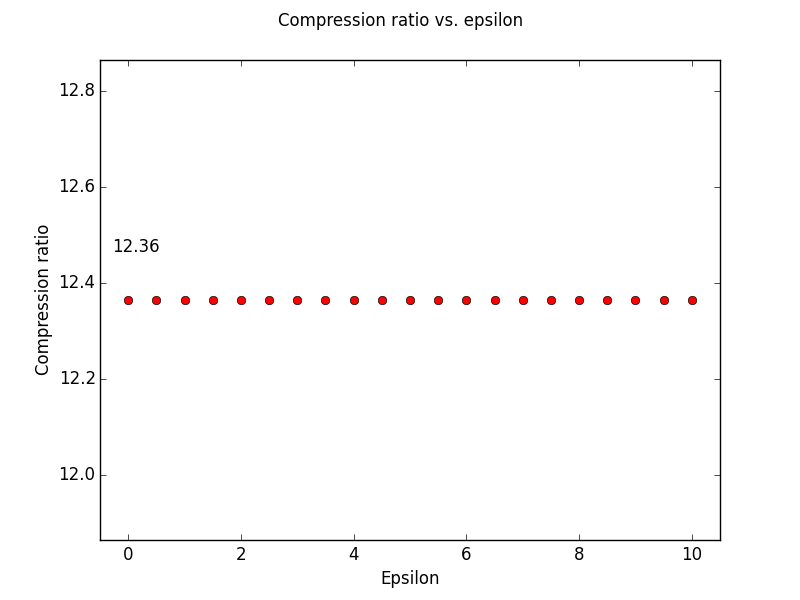
\includegraphics[width=1.0\textwidth]{../graphs/compression_ratio_epsilon.png}
\caption{\label{fig:cr_epsilon} Razón de compresión media con respecto a $\epsilon$ utilizando 30 muestras.}
\end{figure}

\begin{figure}[H]
\centering
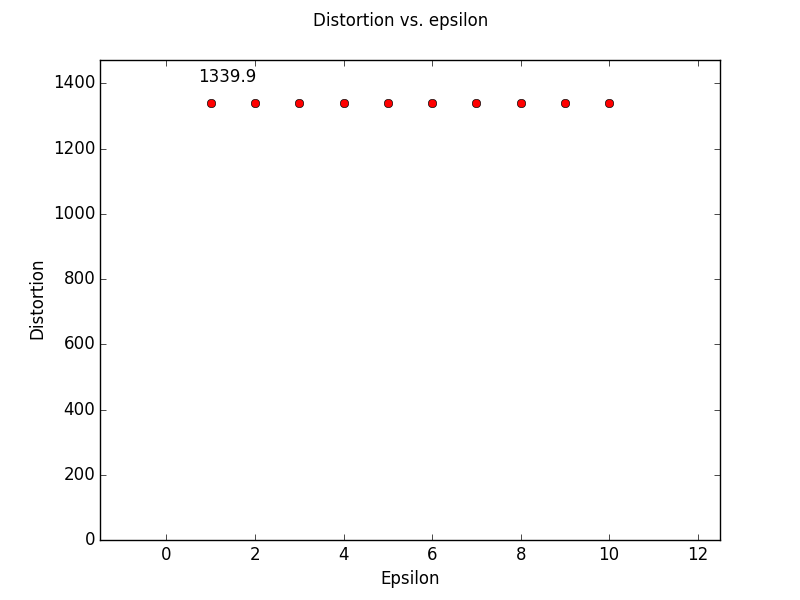
\includegraphics[width=1.0\textwidth]{../graphs/distortion_epsilon.png}
\caption{\label{fig:distortion_epsilon} Distorsión media con respecto a $\epsilon$ utilizando 30 muestras.}
\end{figure}

	Como se puede observar en los gráficos, no se notaron diferencias en razón de compresión media y la distorsión media al variar epsilon entre $0.5$ y $10$. Esto se debe a que en los casos probados, los coeficientes eran muy grandes, por lo que su módulo, era significativamente superior a 10. Por lo tanto, ningún coeficiente fue reemplazado por $0$ ya que ninguno  cumplía con la condición de su módulo sea menor que $\epsilon$.
    
\subsubsection{Gráficos con respecto a L}
Los gráficos fueron obtenidos utilizando $\epsilon = 0.1$ y $L$ entre $1$ y $8$.
\begin{figure}[H]
\centering
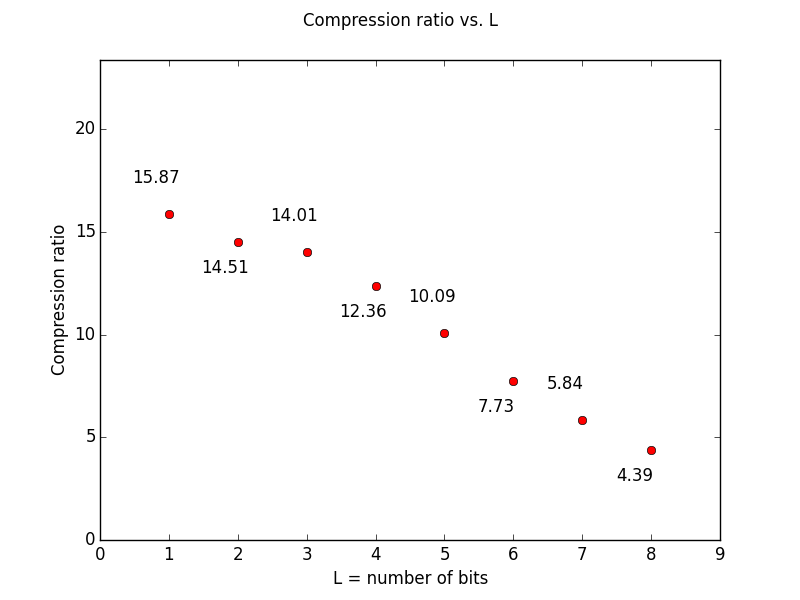
\includegraphics[width=1.0\textwidth]{../graphs/compression_ratio_L.png}
\caption{\label{fig:cr_epsilon} Razón de compresión media con respecto a $L$ utilizando 30 muestras.}
\end{figure}

\begin{figure}[H]
\centering
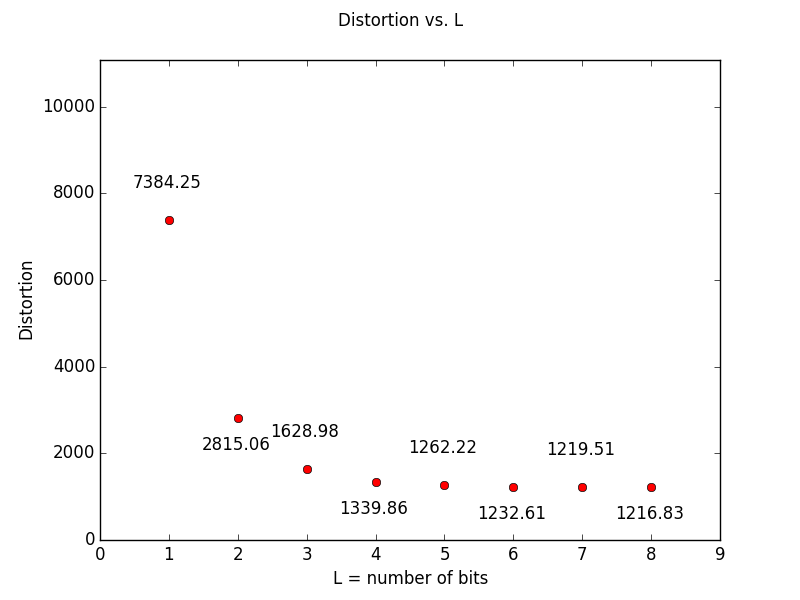
\includegraphics[width=1.0\textwidth]{../graphs/distortion_L.png}
\caption{\label{fig:distortion_L} Distorsión media con respecto a $L$ utilizando 30 muestras.}
\end{figure}

Como se puede observar en los gráficos, a medida que aumenta la cantidad de bits usada para codificar las muestras, disminuye la distorsión y la razón de compresión. La razón de compresión disminuye ya que se utilizan más bits para codificar las muestras, por lo que se utilizan más símbolos y codificaciones más largas. Por lo tanto el tamaño final es mayor. La distorsión disminuye debido a que como se utilizan más bits para codificar las muestras, cuando estás se cuantifican, se obtiene una mayor cantidad de símbolos. Entonces, la distancia que necesitan tener dos coeficientes entre ellos para ser mapeados al mismo entero disiminuye, es decir, hay menores probabilidades de que dos coeficientes sean mapeados al mismo número. Cuando dos coeficientes distintos son mepeados al mismo número, hay pérdida de información. Al disminuir la probabilidad de que dos números sean mepeados al mismo entero, se disminuye la pérdida de información.

\section{Posibles mejoras}

Una mejora que podría ser implementada para mejorar la funcionalidad de trabajo es la habilidad de guardar y cargar datos comprimidos utilizando Huffman.  Se podría diseñar un formato de archivo que almacene el valor máximo y mínimo de los coeficientes obtenidos vía FFT, las asociaciones de símbolo a codigo, y la serie de códigos representando los valores cuantificados.  Una vez creado el archivo, sería posible entonces cargarlo en memoria, y aplicar las operaciones inversas descritas anteriormente para recuperar el sonido almacenado, con cierta pérdida de información.

Otra mejora posible sería optimizar el paso de FFT.  En la documentación de \textbf{fft} de NumPy, se menciona que el la función resulta más performante cuando la cantidad de muestras $N$ es una potencia de 2.  Por lo tanto, se podrían hacer dos cambios al trabajo para manejar casos en donde $N$ no es potencia de 2: agregar muestras nulas al conjunto de muestras hasta que $N = 2^k$, o separar el conjunto de muestras en grupos de tamaño $2^m$, y procesar cada grupo individualmente.


\clearpage

\renewcommand\refname{Referencias}
\begin{thebibliography}{9}

\bibitem{wave}
  Scott Wilson,
  WAVE PCM soundfile format,
  \url{https://ccrma.stanford.edu/courses/422/projects/WaveFormat/}

\bibitem{rajesh}
  G. Rajesh, A. Kumar and K. Ranjeet,
  \emph{Speech Compression using Different Transform Techniques}.
  Indian Institute of Information Technology, Design \& Manufacturing Jabalpur

\bibitem{rosetta}
  Rosetta Code,
  Huffman Coding - Python,
  \url{http://rosettacode.org/wiki/Huffman_coding#Python}

\end{thebibliography}

\end{document}